\documentclass[tikz, border=10pt]{standalone}
\usepackage{amsmath}


% 1. Use the standard Computer Modern Sans Serif
\usepackage[T1]{fontenc}
\renewcommand{\familydefault}{\sfdefault}

\begin{document}
    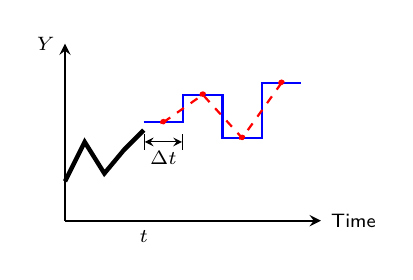
\begin{tikzpicture}[>=stealth, scale=0.5]
        % Axes
        \draw[->, thick] (0,0) -- (6.5,0) node[right] {\scriptsize Time};
        \draw[->, thick] (0,0) -- (0,4.5) node[left] {\scriptsize $Y$};

        % 1. Historical Data
        \draw[ultra thick] (0, 1) -- (0.5, 2) -- (1, 1.2) -- (1.5, 1.8) -- (2, 2.3);
        \node[below] at (2,0) {\scriptsize $t$};

        % 2. Uncertainty Bounds
        %\draw[dashed, gray] (2, 2.5) to[out=30, in=180] (4, 4) -- (6, 4.2);
        %\draw[dashed, gray] (2, 2.5) to[out=-60, in=180] (4, 0.5) -- (6, 0.3);

        % 3. Piecewise Constant (Zero-Order Hold)
        \draw[blue, thick] (2, 2.5) -| (3, 3.2) -| (4, 2.1) -| (5, 3.5) -- (6, 3.5);
        
        % 4. Midpoint Trace (Using the plot command)
        % This replaces the 'marker' option error
        \draw[red, thick, dashed] plot[mark=*, mark options={fill=red, scale=0.8}] coordinates {
            (2.5, 2.5) (3.5, 3.2) (4.5, 2.1) (5.5, 3.5)
        };

        % Interval Label
        \draw[|<->|] (2, 2) -- (3, 2) node[midway, below] {\scriptsize $\Delta t$};
    \end{tikzpicture}
\end{document}